\section{Reševanje enačb}
\label{pogl:enacbe}

\textcolor{red}{popravi da so captioni slik, ki so v več kot eni vrstici, poravbnani na sredini}

Zapustimo deloma področje geometrije in si poglejmo, kako lahko s prepogibanjem papirja rešujemo enačbe z racionalnimi koeficienti.

Spomnimo se še, da smo origami števila definirali kot vsa števila, ki jih lahko s prepogibanjem konstruiramo preko na začetku danega izhodišča $O$ in števila $1$ na realni osi (definicija~\ref{def:origami_stevilo}). V evklidski ravnini (ki je v bijekciji s kompleksno ravnino, dano v definiciji) bomo konstruirali rešitve naših enačb, da pa bo pregibov čim manj in s tem preglednost večja, za označbo pomožnih točk in premic dopuščamo uporabo pisala (saj bi jih tako ali tako znali konstruirati s pregibi).

Začnimo z najbolj osnovno, t.\ j.\ linearno enačbo. Enačba $ax + b = 0$, kjer $a, b \in \Q$ in $a \neq 0$ ima rešitev $x = -b/a$, ki je racionalno število, torej origami število in samo po sebi konstruktibilno. Če bi želeli rešitev konstruirati geometrijsko preko pregibov, v ravnini prepognemo premico $y = ax + b$ (napravimo pregib npr.\ skozi točki (0, b) in (1, a+b)) in njeno presečišče z abscisno osjo nam da iskano rešitev.

Uporaba origamija je za reševanje linearne enačbe očitno manj praktična kot računanje rešitve. Bolj zanimivo je reševanje kvadratne in kubične enačbe. Ker za njune rešitve obstajata splošni formuli, bi jih lahko najprej izračunali in nato preko operacij seštevanja, odštevanja, množenja, deljenja in korenjenja konstruirali s prepogibanjem, vendar je to časovno preveč potratno. Pogledali si bomo, kako se z origamijem lahko temu izognemo in rešitev konstruiramo brez uporabe računskih operacij.

Ključno vlogo bosta v nadaljevanju odigrali origami operaciji~\ref{op:O6} in~\ref{op:O7}. Prva nam hkrati s konstrukcijo tangente na parabolo določi tudi točko na paraboli, skozi katero je pregib tangenten na stožnico, to pa je ekvivalentno reševanju kvadratne enačbe. Druga s konstrukcijo skupne tangente na dve paraboli omogoča reševanje kubične enačbe. Alperin v~\cite[str.\ 129]{alperin2000} pokaže, kako izpeljati koeficient skupne tangente na dani paraboli in izkaže se, da je iskani koeficient rešitev kubične enačbe. Število skupnih tangent je torej enako številu rešitev kubične enačbe, kar pomeni, da imata paraboli v evklidski ravnini največ tri skupne tangente.

V teoriji bi nam prepogibanje papirja pomagalo tudi pri reševanju kvartičnih enačb, saj zanje še obstaja splošna formula (vendar zaradi dolžine praktično neuporabna) in tudi vemo, da lahko enačbo četrte stopnje prevedemo na enačbe nižje stopnje (gl.\ \cite{wikiquartic}, \cite{quartics2012}). Geometrično pa je to reševanje potem težje izvedljivo in zato manj motivacijsko, saj bi postopek reševanja zahteval veliko več pregibov kot pri reševanju ene kubične ali kvadratne enačbe, pa tudi vmesne rezutate bi morali računati. Tako bi se lahko tu z reševanjem enačb preko origamija ustavili, vendar obstajajo alternativne rešitve. V~\cite{edwards2001} je opisan postopek, ki preko \textcolor{red}{projektivne geometrije in dualnih stožnic} ter z Belochinim pregibom reši splošno kubično in nato tudi kvartično enačbo neke določene oblike. Postopek si bomo tudi sami pogledali, saj je zelo zanimiv iz vidika projektivne geometrije.

Za enačbe pete in višjih stopenj pa splošna formula za rešitve ne obstaja več (\emph{Abel-Ruffinijev} izrek, gl.\ \cite{mrinal2019}). Kljub temu se da z origamijem še vedno konstruirati rešitve nekaterih enačb višjih stopenj, vendar ne obstaja postopek z enkratnimi prepogibi -- potrebno se je poslužiti dvojnih (\emph{two fold}) ali večkratnih (\emph{multi-fold}) prepogibov (gl.\ poglavje~\ref{pogl:multifold}).

\subsection{Reševanje kvadratne enačbe preko tangente na parabolo}
\label{podpogl:kvadratna_enacba}

Rešujemo enačbo oblike
$$ a x^2 + b x + c = 0, $$
kjer so $a, b, c \in \Q$ in velja $a \neq 0$.  Njeni splošni rešitvi sta
$$ x_{1,2} = \frac{-b \pm \sqrt{b^2 - 4ac}}{2a}.$$

Postopek, ki si ga bomo pogledali v nadaljevanju, predpostavlja $a = 1$. Ker je vodilni koeficient neničeln, lahko z njim enačbo delimo in pri tem še vedno dobimo racionalne koeficiente, zato lahko predpostavko brez škode za splošnost sprejmemo. Nova oblika enačbe je tako
\begin{equation}
    \label{eq:spl_kv_en}
    x^2 + bx + c = 0.
\end{equation}
Predpostavimo, da ima enačba dve različni realni rešitvi oz.\ da je diskriminanta enačbe pozitivna, t.\ j.\ $D = b^2 - 4c > 0$. Če realnih ničel ni, o origami konstrukciji rešitev namreč nima smisla razpravljati. Če je rešitev ena, je podana kot $x = -b/2$, kar je origami-konstruktibilno število in se ga lahko takoj konstruira.

Enačba~\ref{eq:spl_kv_en} nam poda pokončno parabolo $y = x^2 + bx + c$ z vodoravno premico vodnico in dvema ničlama, ki sta rešitvi naše enačbe. Iščemo absciso presečišča parabole z abscisno osjo.

Zopet se bomo poslužili dosedanjega znanja o operaciji~\ref{op:O6}. Ta nam s pregibom skozi dano točko $B$, ki točko $A$ položi na premico $a$, konstruira tangento na parabolo z goriščem v točki $A$ in premico vodnico $a$.

Naša parabola je z enačbo seveda natančno določena. Ideja iskane konstrukcije rešitev enačbe je določiti tako točko $B$ (najlažje kar na osi parabole), da bi nam izvedba operacije~\ref{op:O6} podala tangento na parabolo ravno v njeni ničli. Želeni pregib mora potekati skozi točko $B$ in gorišče $A$ položiti na tisto točko $A'$ na premici vodnici $a$, ki ima enako absciso kot ničla parabole. (gl.\ sliko~\ref{fig:tockaB_in_O6}). Taka točka $B$ je z osjo parabole in katerokoli izmed ničlama (zaradi simetrije) natanko določena.

\begin{figure}[h]
    \centering
    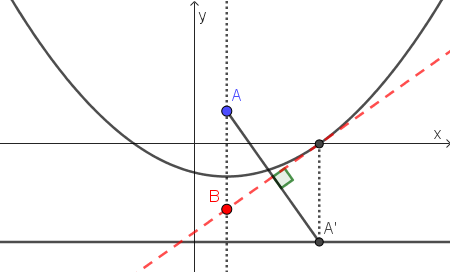
\includegraphics[width=0.5\textwidth]{images/kvadratna_enacba/tockaB_in_O6.png}
    \caption[Iskanje točke $B$]{Operacijo~\ref{op:O6} skozi iskano točko $B$ poda rešitev kvadratne enačbe.}
    \label{fig:tockaB_in_O6}
\end{figure}

Edina nevarnost, da ta konstrukcija ne bo delovala, je možnost, da točka $B$ kdaj ne bo origami-konstruktibilna točka. Zato sedaj izračunajmo njene koordinate in se prepričajmo, da se to nikoli ne bo zgodilo.

Najprej iz dane enačbe parabole določimo njeno gorišče $A$ in premico vodnico $a$. Spomnimo se, da iz enačbe parabole oblike
$$ (x - x_0)^2 = 2p(y - y_0) $$
takoj razberemo koordinati gorišča $(x_0, y_0)$ in enačbo premice vodnice $y = y_0 - p$. V našem primeru enačbo $y = x^2 + bx + c$ preoblikujemo v
$$ \left(x-\left(-\frac{b}{2}\right)\right)^2 = 2 \cdot \frac{1}{2} \left(y - \left(c - \frac{b^2}{4}\right)\right). $$
S tem sta gorišče $A$ in premica vodnica $a$ določena:
$$ A\left(-\frac{b}{2}, c - \frac{b^2 - 1}{4}\right) \text{ in } a: y = c - \frac{b^2 + 1}{4}. $$

Naj bo $t$ ena izmed rešitev enačbe~\ref{eq:spl_kv_en}. Na premici $a$ z $A'$ označimo točko z absciso $t$. Poiščimo enačbo pregiba, ki gorišče $A$ položi v točko $A'$. Ta pregib bo tangenten na parabolo ravno v njeni ničli, njegovo presečišče z osjo parabole $ x = -b/2 $ pa nam bo določilo točko $B$.

Koeficient nosilke daljice $AA'$ je $ - 1/(2t + b)$, torej je koeficient pregiba $k = 2t + b$. Pregib je po konstrukciji tangenten na parabolo v ničli $(t, 0)$, torej je njegova enačba
$$ y = (2t + b)(x - t) = (2t + b)x - 2t^2 - bt = (2t + b)x - t^2 + c. $$
Pri tem smo upoštevali, da velja $t^2 + bt + c = 0$. Presečišče pregiba in osi parabole je tako točka $B$ z absciso $ x = -b/2 $ in ordinato
$$ y = (2t + b)\left(-\frac{b}{2}\right) - t^2 + c = - t^2 - tb + c - \frac{b^2}{2} = c + c - \frac{b^2}{2} = 2c - \frac{b^2}{2}.$$
Obe koordinati sta racionalni, torej je točka $B$ konstruktibilna točka. Ker leži na osi parabole, nam poda obe rešitvi enačbe -- pregiba sta si simetrična glede na os. Povzemimo sedaj postopek konstrukcije rešitve kvadratne enačbe~\ref{eq:spl_kv_en}:
\begin{enumerate}
    \item V koordinatnem sistemu označimo gorišče $A\left(-\frac{b}{2}, c - \frac{b^2}{4} + \frac{1}{4}\right)$, premico vodnico $a: y = c - \frac{b^2 + 1}{4}$ in točko $B(-\frac{b}{2}, 2c - \frac{b^2}{2})$.
    \item Z operacijo~\ref{op:O6} naredimo pregib skozi točko $B$, ki točko $A$ položi na premico $a$ (če je diskriminanta enačbe pozitivna, sta možna pregiba dva).
    \item Skozi sliko točke $A$ naredimo vertikalen pregib in abscisa njegovega presečišča z abscisno osjo je ničla dane enačbe.
\end{enumerate}

\textbf{Primer:} Poiščimo rešitve enačbe $x^2 - x - 1 = 0$. Določimo obe točki in premico: $A(\frac{1}{2}, -1)$, $B(\frac{1}{2}, -\frac{5}{2})$ in $a: y = -\frac{3}{2}.$. Opravimo operacijo~\ref{op:O6} in označimo presečišče abscisne osi in pravokotnice nanjo skozi sliko točke $A$. Če smo bili pri pregibanju natančni, dobimo presečišči pri $x_{1,2} = \frac{1 \pm \sqrt{5}}{2}$ (gl.\ sliko v~\cite[str.\ 37]{hull2020}).

To še zdaleč ni edini postopek za reševanje kvadratne enačbe. Kot še en lep primer Hull v~\cite[str.\ 38]{hull2020} navaja Lillovo konstrukcijo preko krožnice, lahek dokaz pa je prepuščen bralcu. Hkrati je to primer, kako za rešitev nekega problema najprej najdemo (bolj domačo) evklidsko konstrukcijo, ki jo lahko nato preko origami operacij preobrazimo v origami konstrukcijo -- saj že vemo, da lahko s prepogibanjem papirja konstruiramo vse in še več, kar se da z evklidskim orodjem. Pri obravnavi kubične enačbe bomo spoznali Belochino metodo, ki se jo da aplicirati tudi na kvadratno enačbo, in prilagojen postopek je tako opisan v razdelku~\ref{podpodl:kvadr_en_lill}.

\subsection{Lillova metoda in Belochin pregib}
\label{podpogl:kubicna_enacba}

V tem poglavju se bomo spoznali z Lillovo metodo, s katero lahko v teoriji rešimo enačbo poljubne stopnje. V središču naše pozornosti bo origami postopek za reševanje kubične enačbe, ki ga je odkrila že večkrat omenjena Belocheva, vendar se da po Lillovi metodi z uporabo operacije~\ref{op:O6} rešiti tudi kvadratno enačbo, kar si bomo tudi na hitro pogledali proti koncu razdelka. Poleg tega bomo spoznali tudi več sadov Belochinega pregiba.

Sedaj pa vzemimo enačbo oblike
$$ a x^3 + b x^2 + c x + d = 0, $$
kjer so $a, b, c, d \in \Q$ in velja $a \neq 0$. Tu je navedena ena oblika zapisa njene splošne rešitve:

\begin{align*}
    Q &= \sqrt{(2b^3 - 9abc + 27a^2d)^2 - 4(b^2 - 3ac)^3} \\
    C &= \sqrt[3]{\frac{1}{2}(Q + 2b^3 - 9abc + 27a^2d)} \\
    x_1 &= - \frac{b}{3a} - \frac{C}{3a} - \frac{b^2 - 3ac}{3aC} \\
    x_2 &= - \frac{b}{3a} + \frac{C(1 + i\sqrt{3})}{6a} + \frac{(1 - i\sqrt{3})(b^2 - 3ac)}{6aC} \\
    x_2 &= - \frac{b}{3a} + \frac{C(1 - i\sqrt{3})}{6a} + \frac{(1 + i\sqrt{3})(b^2 - 3ac)}{6aC}
\end{align*}

Operacija~\ref{op:O6} nam je preko konstrukcije tangente na parabolo pomagala rešiti kvadratno enačbo. Spomnimo se, da je Belocheva to v 30-ih letih prejšnjega stoletja nadgradila z operacijo~\ref{op:O7}, ki nam konstruira skupno tangento na dve paraboli hkrati. Po njej jo tudi imenujemo \emph{Belochin pregib}. Z njim je kot prva odkrila resnično moč origami konstrukcij, a je žal trajalo več kot pol stoletja, da so matematiki začeli ceniti njeno odkritje.

\subsubsection{Reševanje kubične enačbe z Belochinim postopkom}

Belocheva je sama odkrila naslednjo metodo reševanja kubične enačbe, kjer nam vsak Belochin pregib poda eno izmed rešitev. Iz začetka poglavja že vemo, da je število rešitev enako številu skupnih tangent, torej številu možnih Belochinih pregibov.

Belocheva v svojem postopku izhaja iz Lillove genialne metode iskanja ničel poljubnih polinomov z realnimi koeficienti, ki si jo bomo v naslednjem razdelku podrobneje pogledali, za njeno aplikacijo pa uporabi avtorsko konstrukcijo -- Belochin kvadrat.

\subsubsection*{Lillova metoda}

Njen avtor je avstrijski inženir Eduard Lill, ki jo je l.\ 1867 opisal v svojem članku~\cite{lill1867}. Gre za inovativen postopek, ki je v svoji osnovi čisto enostaven. Imejmo poljuben polinom $ p(x) = a_n x^n + a_{n-1} x^{n-1} + \ldots + a_2 x^2 + a_1 x + a_0 $ z realnimi koeficienti in iščemo njegove realne ničle, če obstajajo. Lill je iz njegovih koeficientov s sledečim postopkom v ravnini ustvaril enolično pot. Običajno se za njeno konstrukcijo uporablja figuro želve, ki nam kaže, v katero smer se premika pa tudi kam je usmerjena.

Na začetku želvo postavimo v koordinatno izhodišče $O$ tako, da gleda v pozitivno smer $x$-osi. Želva najprej v to smer prehodi razdaljo, enako koeficientu $a_n$. Nato se obrne za $90^\circ$ v nasprotno smer urinega kazalca in prehodi naslednjo razdaljo $a_{n-1}$. To ponovi za vsak koeficient polinoma in po prehojeni razdalji $a_0$ se ustavi v neki točki $T$ (slika~\ref{fig:primera_zelve}). Če je kateri od koeficientov negativen, želva hodi ritensko (primer (b) na sliki~\ref{fig:primera_zelve} za koeficiente $a_3, a_2$ in $a_0$), v primeru ničelnega koeficienta pa obstoji na mestu in se samo obrne. S potjo želve dobimo lomljeno črto iz največ $n+1$ daljic, ki jih brez škode označujmo kar z njihovimi ``pripadajočimi'' koeficienti.

\begin{figure}[h]
    \centering
    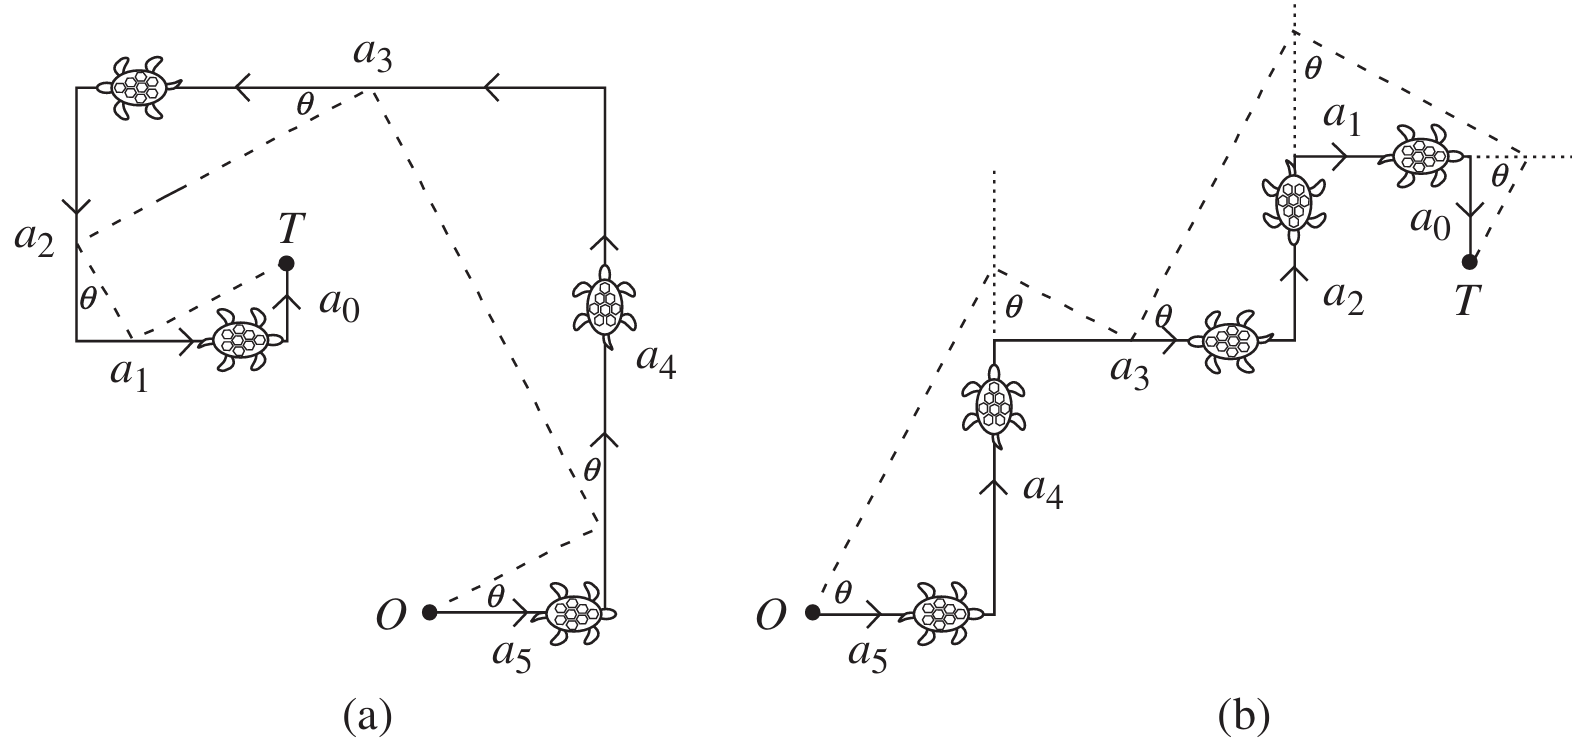
\includegraphics[width=0.9\textwidth]{images/kubična enačba/primera_zelvine_poti.png}
    \caption[Primera želvine poti]{Primera želvine poti za polinoma pete stopnje. Vzeto iz~\cite[str.\ 311]{hull2011}.}
    \label{fig:primera_zelve}
\end{figure}

Sedaj se v izhodišče $O$ postavimo še mi in z laserskim žarkom poskusimo zadeti želvo v točki $T$. Žarek najprej usmerimo daljico $a_{n-1}$, od katere se odbije v daljico $a_{n-2}$, od te v daljico $a_{n-3}$ in tako naprej. (slika~\ref{fig:primera_zelve}). Pri tem upoštevamo troje:
\begin{itemize}
    \item laserski žarek ne upošteva odbojnega zakona in se od daljice vedno odbije pod kotom $90^\circ$, zato so vpadni koti žarka na vse daljice med seboj enaki in prav tako to velja za odbojne kote;
    \item žarek se lahko odbije tudi od nosilke daljice;
    \item vsakič sta možni dve smeri odboja -- na isto stran daljice (oz.\ njene nosilke) ali skoznjo -- izberemo pa tisto, ki nam omogoči, da sploh lahko zadenemo naslednjo daljico.
\end{itemize}
ecimo, da smo zmogli zadeti želvo. Kot, ki ga v točki $O$ oklepata laserski žarek in abscisna os, označimo z $\theta$.

\begin{trditev}
    $x_{\theta} = - \tan \theta$ je ničla polinoma $p(x)$.
\end{trditev}

\begin{dokaz}
    Vzemimo primer, ko so vsi koeficienti polinoma $p(x)$ pozitivni. Želvina pot je v tem primeru sestavljena iz $n+1$ daljic, pot laserskega žarka (ki se vedno odbije od daljice in ne njene nosilke) pa iz $n$ daljic. Slednje so ravno hipotenuze pravokotnih trikotnikov. Za vsako od njih je nasprotna kateta kota $\theta$ del daljice $a_i$, priležno kateto pa označimo z $y_i$ ($ n \geq i \geq 1$). dobimo
    \begin{align*}
        y_n &= \tan \theta \cdot a_n = - x_{\theta} a_n \\
        y_{n-1} &= \tan \theta \cdot (a_{n-1} - y_n) = - x_{\theta} (a_{n-1} + x a_n) = - (a_{n-1} x_{\theta} + a_n x_{\theta}^2)\\
        y_{n-2} &= \tan \theta \cdot (a_{n-2} - y_{n-1}) = - x_{\theta} (a_{n-2} + a_{n-1} x_{\theta} + a_n x_{\theta}^2) = \\
        &= - (a_{n-2} x_{\theta} + a_{n-1} x_{\theta}^2 + a_n x_{\theta}^3) \\
        &\vdots \\
        y_1 &= - (a_1 x_{\theta} + a_2 x_{\theta}^2 + \ldots + a_{n-1} x_{\theta}^{n-1} + a_n x_{\theta}^n).
    \end{align*}
    V zadnji enakosti desno stran premaknimo na levo in upoštevamo $y_1 = a_0$. Dobimo ravno $p(x_{\theta}) = 0$, torej je $x_{\theta} = - \tan \theta$ res ničla tega polinoma.

    \textcolor{red}{Primer negativnih koeficientov:~\cite[str.\ 36]{zore2022}.}

    \textcolor{red}{Primer ničelnih koeficientov: isto kot prej, samo se spusti $y_i$ za tisti $i$, za katerega je $a_i = 0$. (\textcolor{red}{???})}
\end{dokaz}

Če pod nobenim kotom $\theta$ ne moremo zadeti želve, je polinom $p(x)$ brez realnih ničel.

Pojavi se nam vprašanje, kako določiti kot $\theta$. Za polinom tretje stopnje je Belocheva preko svojega pregiba našla zelo preprosto rešitev, ki si jo bomo sedaj pogledali.

\subsubsection*{Belochin kvadrat}

Imejmo dani točki $A$ in $B$ ter premici $r$ in $s$. Z origamijem konstruirajmo kvadrat $WXYZ$, kjer oglišče $X$ leži na premici $r$, njegovo sosednje oglišče $Y$ pa na premici $s$. Velja še, da točka $A$ leži na stranici $WX$ (ali njeni nosilki), točka $B$ pa na stranici $ZY$ (ali njeni nosilki, slika~\ref{fig:beloch_kvadrat}).

\begin{figure}[h]
    \centering
    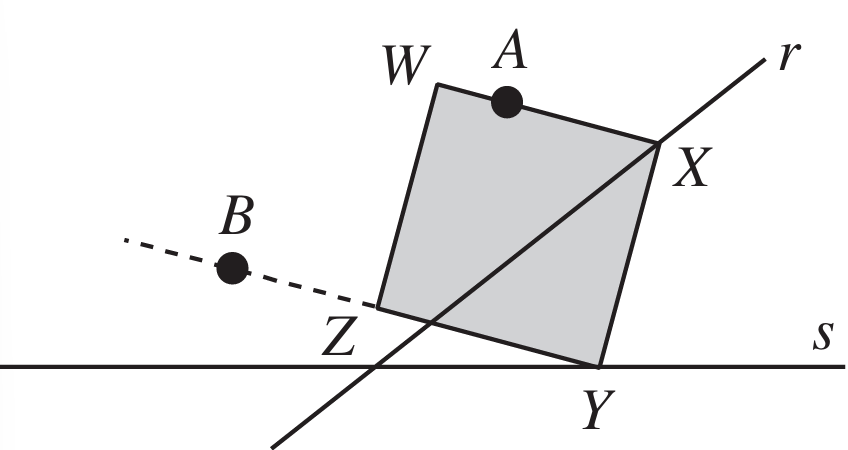
\includegraphics[width=0.4\textwidth]{images/kubična enačba/beloch_kvadrat.png}
    \caption[Belochin kvadrat]{Belochin kvadrat. Vzeto iz~\cite[str.\ 309]{hull2011}.}
    \label{fig:beloch_kvadrat}
\end{figure}

Belocheva je iznašla naslednji postopek, ki nam konstruira ta kvadrat:
\begin{itemize}
    \item Najprej konstruiramo premico $r'$, ki je vzporedna premici $r$ in od nje enako oddaljena kot točka $A$, tako da premica $r$ leži med točko $A$ in premico $r'$. Na enak način premici $s$ konstruiramo njeno vzporednico $s'$ (slika~\ref{fig:beloch_kvadrat_konstrukcija} levo). To konstrukcijo opravimo s prepogibi iz operacije~\ref{op:O5}, zrcaljenja točke čez premico ter ponovne uporabe operacije~\ref{op:O5}. Zaradi preglednosti seveda dopuščamo, da namesto zrcaljenja preprosto prepognemo po premici in s svinčnikom označimo sliko točke.
    \item Nato opravimo Belochin pregib, ki točko $A$ slika v točko $A'$ na premici $r'$, točko $B$ pa v točko $B'$ na premici $s'$ (slika~\ref{fig:beloch_kvadrat_konstrukcija} na sredi).
    \item Naj bo točka $X$ središče daljice $AA'$ in točka $Y$ središče daljice $BB'$. Ker je pregib simetrala teh dveh daljic $AA'$ in $BB'$, sta njuni središči po konstrukciji\footnote{Gledamo lahko dva podobna pravokotna trikotnika s skupnim ogliščem v točki $A$ (oz.\ $B$), enega dvakrat večjega od drugega} ravno presečišči pregiba s premicama $r$ in $s$ (slika~\ref{fig:beloch_kvadrat_konstrukcija} desno).
    \item Daljica $XY$ -- ena izmed stranic kvadrata -- je po konstrukciji pravokotna na daljici $AX$ in $BY$, zato samo še določimo točki $W$ in $Z$ na daljicah ali njunih nosilkah in tako dobimo Belochin kvadrat.
\end{itemize}

\begin{figure}[h]
    \centering
    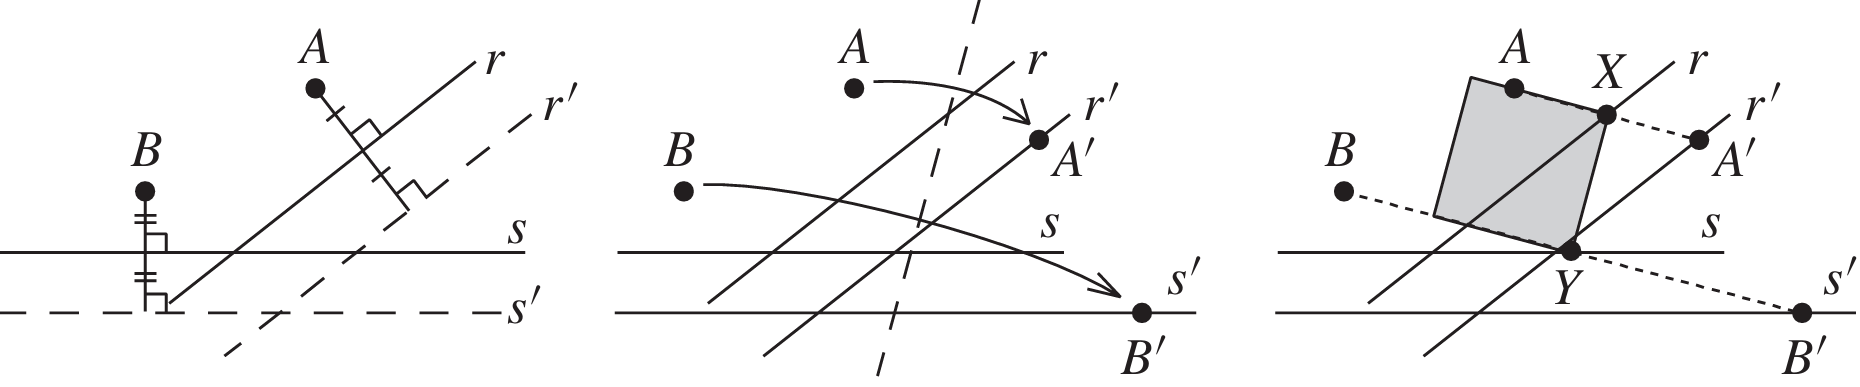
\includegraphics[width=0.95\textwidth]{images/kubična enačba/beloch_kvadrat_konstrukcija.png}
    \caption[Konstrukcija Belochinega kvadrata]{Konstrukcija Belochinega kvadrata z origamijem. Vzeto iz~\cite[str.\ 310]{hull2011}.}
    \label{fig:beloch_kvadrat_konstrukcija}
\end{figure}

\subsubsection*{Konstrukcija $\sqrt[3]{2}$ z Belochinim kvadratom}
\label{podpogl:beloch_kvadrat_koren}

Preden ravno naučeno znanje uporabimo za reševanje kubičnih enačb, si še na hitro poglejmo, kako lahko tudi z Belochinim kvadratom rešimo starogrški problem podvojitve kocke.

Za premico $r$ vzemimo ordinatno os, za premico $s$ pa abscisno os. Določimo še $A = (-1,0)$ in $B = (0, -2)$. Vzporednici sta torej $r': x = 1$ in $s': y = 2$. Belochin pregib seka premico $r$ v točki $X$, premico $s$ pa v točki $Y$ (slika~\ref{fig:beloch_koren}). Z $O$ označimo koordinatno izhodišče in opazimo podobne pravokotne trikotnike $OAX$, $OXY$ in $OYB$. Z upoštevanjem $|AO| = 1 $ in $|OB| = 2$ dobimo sledeča razmerja:
$$ \frac{|OX|}{|AO|} = \frac{|OY|}{|OX|} = \frac{|OB|}{|OY|} \Longrightarrow |OX| = \frac{|OY|}{|OX|} = \frac{2}{|OY|}, $$
iz česar sledi
$$ |OX|^3 = |OX| \cdot \frac{|OY|}{|OX|} \cdot \frac{2}{|OY|} = 2 \Longrightarrow |OX| = \sqrt[3]{2}. $$

\begin{figure}[h]
    \centering
    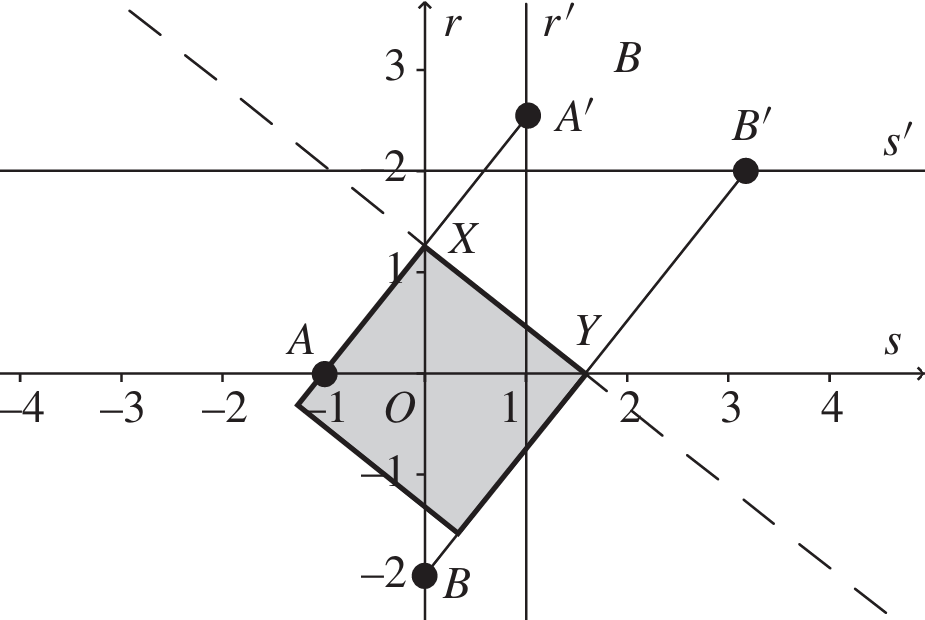
\includegraphics[width=0.5\textwidth]{images/kubična enačba/beloch_koren.png}
    \caption[Konstrukcija kubičnega korena števila dva]{Konstrukcija $\sqrt[3]{2}$ preko Belochinega kvadrata. Vzeto iz~\cite[str.\ 310]{hull2011}.}
    \label{fig:beloch_koren}
\end{figure}

Vidimo lahko, da je to enaka konstrukcija kot jo je 50 let kasneje neodvisno od Belocheve odkril G.\ Martin (razdelek~\ref{podpogl:podvojitev_kocke}), le da je za točko $B$ vzel točko $(0, -k)$ in s tem konstruiral dolžino $\sqrt[3]{k}$ za poljuben origami-konstruktibilen $k$.

\subsubsection*{Združitev Lillove metode in Belochinega kvadrata}

Za poljubno enačbo $a x^3 + b x^2 + c x + d = 0$, kjer $ a \neq 0$, povežimo sedaj Lillovo metodo s konstrukcijo primernega Belochinega kvadrata, ki nam bo natančno določil kot $\theta$. Postopek je sledeč (gl.\ tudi sliko~\ref{fig:beloch_kubicna_resitev}):

\begin{enumerate}
    \item Za točko $A$ vzemimo izhodišče $O$. Začrtamo želvino pot za polinom $p(x) = a x^3 + b x^2 + c x + d$, ki se začne v točki $A$ in konča v točki $B$. V primeru neničelnih koeficientov je pot sestavljena iz štirih stranic, pot laserskega žarka pa iz treh.
    \item Premica $r$ naj bo nosilka daljice $b$ ($r: x = a$), premica $s$ pa nosilka daljice $c$ ($s: y = b$).
    \item Določimo premici $r': x = 2a$ in $s': b + d$ ter opravimo Belochin pregib, ki točko $A$ položi na premico $r'$ in točko $B$ na premico $s'$.
    \item Presečišči pregiba s premicama $r$ in $s$ zaporedoma označimo s točkama $X$ in $Y$.
    \item Zarišemo daljice $AX$, $XY$ in $YB$.
\end{enumerate}

Ker po konstrukciji velja $ AX \perp XY \perp YB $, je to iskana pot laserskega žarka, ki se odbija pod pravim kotom in zadene želvo. Kot $\theta$ je kot, ki ga oklepata daljici $a_3$ in $AX$. Rešitev je torej $x_{\theta} = - \tan \theta$.

\begin{figure}[h]
    \centering
    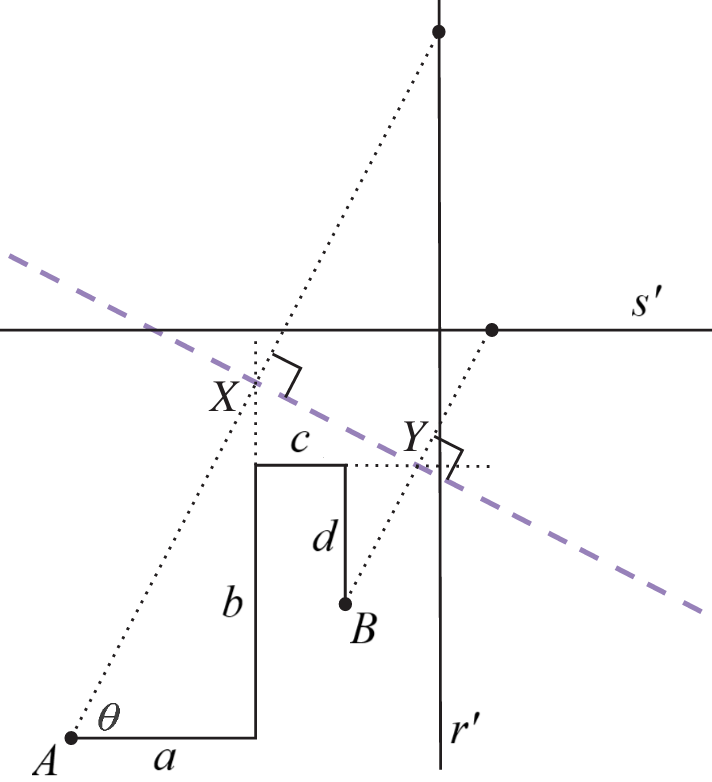
\includegraphics[width=0.4\textwidth]{images/kubična enačba/beloch_kubicna_resitev.png}
    \caption[Lillova metoda z Belochinim kvadratom]{Konstrukcija želvine poti za Lillovo metodo preko Belochinega kvadrata. Vzeto in preurejeno iz~\cite[str.\ 313]{hull2011}.}
    \label{fig:beloch_kubicna_resitev}
\end{figure}

Če ima enačba še dve realni rešitvi, sta možna tudi še dva Belochina pregiba (enačba namreč ne more imeti dveh realnih rešitev, saj kompleksne rešitve nastopajo v konjugiranih parih).

\opomba{V resnici nikoli do sedaj nismo potrebovali konstruirati celega kvadrata; potrebovali smo le stranico $XY$ in dejstvo, da je pregib pravokoten na daljici $AX$ in $BY$.}

\opomba{Enačbe premic $r, s, r'$ in $s'$ so univerzalne in zgornja konstrukcija tako deluje tudi v primeru, ko je kakšen od koeficientov $b, c, d$ ničeln.}

Za konkretne primere uporabe Belochinega postopka za reševanje kubičnih enačb glej~\cite[38--44]{zore2022}.

Kot zanimivost Lavričeva v~\cite[str.\ 10--13]{lavric2013} s postopkom, ki je malo preurejen Belochin postopek, še analitično pokaže, da je ob primerno izbranih točkah $A$ in $B$ ter premicah $r$ in $s$ koeficient tangentnega pregiba rešitev kubične enačbe. Točki in premici izbere tako, da sta točki $X$ in $Y$ ravno presečišči z ordinatnima osema, iz česar lahko takoj razberemo koeficient tangente. V dokazu izpelje enačbi pripadajočih parabol in splošno enačbo njunih tangent ter iz tega dokaže rečeno. To je lahko odlična vaja za dijake, ki si želijo kakšnega izziva.

\subsubsection{Reševanje kvadratne enačbe z Lillovo metodo}
\label{podpodl:kvadr_en_lill}

Lillovo lahko uporabimo tudi za reševanje kvadratne enačbe $a x^2 + b x + c = 0, a \neq 0$. Na enak način v koordinatni sistem zarišemo želvino pot, ki se začne v točki $A$ in konča v točki $B$. Za razliko od prej tu ne uporabimo Belochinega pregiba, temveč pregib iz operacije~\ref{op:O6}. Namesto dveh premic $r$ in $s$ imamo le eno -- naj bo $r$ nosilka daljice $b$. Kot prej -- na razdalji $a$ na drugi strani točke $A$ -- označimo še njeno vzporednico $r'$. Konstruiramo pregib, ki gre skozi točko $B$ in točko $A$ položi na premico $r'$. Njegovo presečišče s premico $r$ nam določi točko $X$, kjer se žarek iz točke $A$ pod pravim kotom odbije v točko $B$. Na sliki~\ref{fig:kv_en_lill} je primer kosntrukcije pri negativnem koeficientu $c$. S tem je kot $\theta$ določen. Premislili smo tudi že, da sta možna največ dva pregiba in da je število pregibov enako številu realnih rešitev enačbe.

\begin{figure}[h]
    \centering
    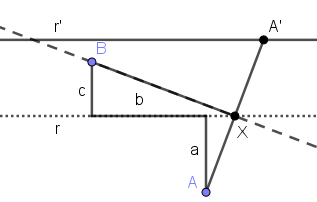
\includegraphics[width=0.5\textwidth]{images/kvadratna_enacba/kvadratna_enacba_lillova_metoda.png}
    \caption[Lillova metoda za kvadratno enačbo]{Reševanje kvadratne enačbe po Lillovi metodi z operacijo~\ref{op:O6} ($c < 0$).}
    \label{fig:kv_en_lill}
\end{figure}

\subsubsection{Hatorijeva konstrukcija}

Japonski matematik Koshiro Hatori navaja postopek, ki je zelo podoben Belochinem postopku, vendar ga je avtor iznašel neodvisno od Belochinega dela. Brez škode za splošnost predpostavi $a = 1$ in za reševanje enačbe $x^3 + bx^2 + cx + d = 0$ sledi naslednjim korakom:
\begin{itemize}
    \item Vkoordinatnem sistemu označimo točki $A = (b, 1)$ in $B = (d, c)$ ter premici $a: y = -1$ in $b: x = -d$.
    \item Opravimo pregib, ki točko $A$ položi na premico $a$ ter točko $B$ na premico $b$ (kar je ravno Belochin pregib).
\end{itemize}
Avtor zaključi, da je koeficient opravljenega pregiba rešitev naše enačbe.

Bralec lahko sam premisli, da je to v resnici ravno Belochin postopek, le da se želva na začetku svoje poti ne nahaja v koordinatnem izhodišču in je najprej usmerjena navzdol. Prav tako lahko izrazi koeficient pregiba s kotom ob začetni točki $A$ in res dobi $k = - \tan \theta$. \textcolor{red}{(to si tudi sama preverila in res drži)}. Za geometrijsko razlago preko parabol gl.~\cite{hatori2003}.

\opomba{Seveda bi lahko vzeli katerikoli $a \in \Q$ in vzeli premico $a: y = -a$.}

\subsection{Alperinova rešitev}

\textcolor{red}{Poglej kej sploh to rešuje, kakšne enačbe, če to spada pod Lillovo metodo, dej to kot podpoglavje v prejšnje poglavje (dodaj še en ``sup'')}

\textcolor{red}{Tudi on neodvisno od Belocheve, je pa pri njem $a= 1, b = 0$, kar se da nardit z vsako kubično enačbo, pač z uvedno nove spremenljivke al neki, da se kvadratni člen uniči.} (gl.\ Hull 2020 str.\ 43, hull2013 str.\ 78 spodej) - prevedba kubične enačbe na kvadratno al neki tazga.

\subsection{Kubična in kvartična enačba v afini ravnini}

\textcolor{red}{A je naslov ok ali je preveč misteriozen in kontraverzen?}

Kot že omenjeno v uvodu tega poglavja, se Edwards in Shurman v~\cite{edwards2001} ukvarjata z reševanjem enačb tretje in četrte stopnje preko iskanja skupnih tangent na določene stožnice, pri tem pa uporabljata princip Belochinega pregiba. Pri kubični enačbi iz njenih koeficientov določita gorišči in premici vodnici dveh parabol, rešitve enačbe pa so koeficienti skupnih tangent. Postopek za reševanje kvartične enačbe je podoben, le da iz njenih koeficientov določita parabolo in krožnico, rešitve pa so začetne vrednosti skupnih tangent. Videli bomo, da slednji postopek deluje le za nekatere kvartične enačbe.

Preden se podamo na natančnejšo razčlenitev njunega dela, se najprej vprašajmo, kako lahko z origamijem določimo skupno tangento na parabolo in krožnico -- do sedaj to namreč znamo le v primeru dveh parabol (preko Belochinega pregiba). Postopek je v svojem bistvu zelo enostaven. Pri danem gorišču in premici vodnici parabole ter krožnici s središčem v točki $S$ in polmerom $r$ zarišemo krožnico z istim središčem ter dvakratnim polmerom, torej $2r$. Nato po zgledu Belochinega pregiba opravimo pregib, ki gorišče parabole položi na njeno premico vodnico, središče $S$ pa na rob krožnice s polmerom $2r$. Pregib je tako res skupna tangenta na parabolo in krožnico s polmerom $r$ (slika \textcolor{red}{dej kakšen slikovni primeeeeer -- lahko kar sliko 3 iz tega vira}).

\begin{opomba}
    V tem razdelku za potrebe reševanja izjemoma potrebujemo šestilo, s katerim iz koeficientov kvartične enačbe konstruiramo krožnico.
\end{opomba}

Postopek se trenutno lahko dozdeva enostaven, vendar nas do enačb iskanih stožnic čaka še dolga pot. (\textcolor{red}{Nekej od tega de se moramo spomnit splošne enačbe stožnic in afine pa projektivne geometrije blablabla})

\textcolor{red}{Definicija projektivne geometrije nad vektorskim prostorom V (mi bomo imeli V = $\R^3$.)}

Stožnica $\mathcal{S}$ ima v $\mathcal{P}(\R^3)$ \textcolor{red}{(A ta``P'' je normalen font al tak kot tle?)} homogenizirano \textcolor{red}{(?)} enačbo
\begin{equation}
    \label{en:stoznica_splosna}
    \mathcal{S}: a_{11}x^2 + 2a_{12}xy + a_{22}y^2 + 2a_{13}xz + 2a_{23}yz + a_{33}z^2 = 0,
\end{equation}
kar lahko zapišemo v obliki
\begin{equation*}
    \mathcal{S}: v^\intercal M v = 0,
    \text{ kjer sta } v =
    \begin{bmatrix}
        x\\
        y\\
        z
    \end{bmatrix}
    \text{ in } M =
    \begin{bmatrix}
        a_{11} & a_{12} & a_{13}\\
        a_{12} & a_{22} & a_{23}\\
        a_{13} & a_{23} & a_{33}
    \end{bmatrix}.
\end{equation*}

Pri tem je simetrična matrika $M$ definirana do neničelnega skalarnega večkratnika natančno. Stožnica $\mathcal{S}$ je \emph{neizrojena} (ni unija dveh premic ali ene, dvojno štete premice), če ima poln rang, t.\ j.\ \textcolor{red}{rang (-- dej v matematično okolje?)} $ M = 3$ oz. ekvivalentno, $\det M \neq 0$. V nadaljevanju bomo delali le z neizrojenimi stožnicami, torej vedno obstaja inverz matrike $M$, ki je prav tako simetričen.

Iz prvega minorja matrike $M$ lahko takoj preberemo, za katero vrsto neizrojene stožnice gre. Naj bo $A_M = a_{11}a_{22} - a_{12}^2$ \textcolor{red}{(Vir tega je Wikipedia: Matrix representation of conic sections. Kakšen bolj zanesljiv vir?)}:
\begin{itemize}
    \item $\mathcal{S}$ je hiperbola, če in samo če $A_M < 0$,
    \item $\mathcal{S}$ je parabola, če in samo če $A_M = 0$ in
    \item $\mathcal{S}$ je elipsa, če in samo če $A_M > 0$. Če poleg tega velja še $a_{11} = a_{22}$ in $a_{12} = 0$, je $\mathcal{S}$ krožnica.
\end{itemize}

\textcolor{red}{(Definicija dualnosti?)}

\textcolor{red}{\emph{Dualno stožnico} (a je prevod ok?)} stožnice $\mathcal{S}$ definiramo z inverzno matriko:
\begin{equation*}
    \mathcal{\hat{S}}: v^\intercal M^{-1} v = 0.
\end{equation*}

Naj bo $p \in \mathcal{S}$ točka na stožnici $\mathcal{S}$ in naj bo $q = Mp$. Potem je
 $$q^\intercal M^{-1} q = (Mp)^\intercal M^{-1} (Mp) = p^\intercal M^\intercal M^{-1} M p = p^\intercal M p = 0,$$
 kar pomeni, da je $q \in \mathcal{\hat{S}}$. Ker je $M$ obrnljiva, je preslikava $\mathcal{S} \longrightarrow \mathcal{\hat{S}}$ s predpisom $p \mapsto Mp$ bijekcija med stožnico $\mathcal{S}$ in njeno dualno stožnico $\mathcal{\hat{S}}$. Kaj pa so točke dualne stožnice $\mathcal{\hat{S}}$? (\textcolor{red}{Dokončaj; zakaj je $q$ ravno tangenta na $\mathcal{S}$?})

 Naj bosta $\mathcal{S}_1$ in $\mathcal{S}_2$ stožnici s pripadajočima simetričnima obrnljivima matrikama $M_1$ in $M_2$. Potem je njuna skupna tangenta skupna točka njunih dualnih stožnic $\mathcal{\hat{S}}_1$ in $\mathcal{\hat{S}}_2$. Torej iščemo $q \in \mathcal{\hat{S}}_1, \mathcal{\hat{S}}_2$, (\textcolor{red}{a je q res prou tangenta? to je pač točka od dualne stožnice}) ki reši sistem enačb
 \begin{equation}
    \label{eq:afin_sistem_tangenta_splosen}
    q^\intercal M^{-1}_1 q = 0 \; \text{ in } \; q^\intercal M^{-1}_2 q = 0.
 \end{equation}
 \textcolor{red}{kakšne oblike je q? oziroma tangenta?}

 \subsubsection*{Reševanje kubične enačbe}

 Zopet rešujemo kubično enačbo oblike $ x^3 + bx^2 + cx + d = 0, d \neq 0$. Za stožnici vzamemo naslednji paraboli:
 \begin{itemize}
    \item $\mathcal{P}_1: (y+c)^2 = -4d(x-b)$ z goriščem $F_1 (b - d, -c)$ in premico vodnico $L_1: x = b + d$,
    \item $\mathcal{P}_2: x^2 = -4y$ z goriščem $F_2 (0, -1)$ in premico vodnico $L_2: y = 1$.
 \end{itemize}

 Iz enačb parabol zapišemo njuni matriki
$$ M_1 =
    \begin{bmatrix}
        0 & 0 & 2d\\
        0 & 1 & c\\
        2d & c & c^2-4bd
    \end{bmatrix}
    \; \text{ in } \; M_2 =
    \begin{bmatrix}
        1 & 0 & 0\\
        0 & 0 & 2\\
        0 & 2 & 0
    \end{bmatrix}
$$
ter izračunamo njuna inverza
$$ M^{-1}_1 = \frac{1}{d}
    \begin{bmatrix}
        b & -c/2 & 1/2\\
        -c/2 & d & 0\\
        1/2 & 0 & 0
    \end{bmatrix}
\; \text{ in } \; M^{-1}_2 =
    \begin{bmatrix}
        1 & 0 & 0\\
        0 & 0 & 1/2\\
        0 & 1/2 & 0
    \end{bmatrix}.
$$

Naj bo $q = [A\;B\; C]^\intercal \in \mathcal{\hat{P}}_1, \mathcal{\hat{P}}_2$ skupna tangenta (\textcolor{red}{je to res ``tangenta'' al kako se temu reče?}) na paraboli $\mathcal{P}_1$ in $\mathcal{P}_2$. Iz sistema enačb~\ref{eq:afin_sistem_tangenta_splosen} dobimo nov sistem
\begin{equation}
    \label{eq:afin_sistem_tangenta_ABC_kub}
    bA^2 - cAB + AC + dB^2 = 0 \; \text{ in } \; -BC = A^2.
\end{equation}

Da dobimo \textcolor{red}{nevertikalno afino skupno} tangento na paraboli $\mathcal{P}_1$ in $\mathcal{P}_2$, normaliziramo $B = -1$ in $z = 1$, s čimer dehomogeniziramo (\textcolor{red}{? poglej kako je z izrazi, pa $z = 1$ je verjetno pač k je afina ravnina, zakaj pa je $B = -1$?}) tangento $Ax + By + Cz = 0$ v $y = Ax + C$. S tem se druga enačba v sistemu~\ref{eq:afin_sistem_tangenta_ABC_kub} preuredi v $C = A^2$, prva pa v
$$ A^3 + bA^2 + cA + d = 0,$$
kar pomeni, da nam $A$, koeficient skupne tangente, reši izvorno kubično enačbo.

\textcolor{red}{Dodaj konkreten primer iz članka, origami pregibe si tudi fizično sprobala na enem listi.}

\subsubsection*{Reševanje kvartične enačbe}

Kot že povedano, sledeči postopek ne rešuje splošne enačbe četrte stopnje, temveč njeno zreducirano obliko
\begin{equation}
    \label{eq:reduc_kvart_ev}
    x^4 + bx^2 + 2cx + d = 0
\end{equation}
(\textcolor{red}{Omeni, da se da vsako kvartično enačbo zreducirat v to?})
Smiselno predpostavimo $d \neq 0$, saj bi se v nasprotnem primeru pri eliminaciji ničle $x = 0$ enačba prevedla na kubično. Poleg tega predpostavimo še $c \neq 0$, ki nam prepreči, da bi se enačba z uvedbo nove spremenljivke za $x^2$ prevedla celo na kvadratno enačbo.

\textcolor{red}{omeni Bezuatov izrek al kaj je že in da dualne stožnice imajo kvadratno enačbo, kar pomeni, da imata dve največ štiri skupne točke (tangente) v kompleksni projektivni ravnini; ker so inverzne matrike realne, nastopajo v konjugiranih parih, torej imata po nič, dve ali štiri skupne tangente (šteto z večkratnostjo). A je tu not tudi tangenta v neskončnosti všteta? Skratka, dve paraboli pa imata skupno tangento v neskončnosti, kar pomeni, da potem ne pustita dovolj afinih tangent, ki bi rešile kvartično enačbo (ker so afine tangente največ tri). Zato ne moremo vzeti dveh parabol.}

Zgornjo metodo bi lahko uporabili tudi tu. Avtorja pri predpostavki $bd - c^2 \neq 0$ vzameta naslednji stožnici:
\begin{itemize}
    \item $\mathcal{S}: dx^2 + 2cxy + by^2 + bd - c^2 = 0$ in
    \item parabolo od prej, t.\ j.\ $\mathcal{P}: x^2 = -4y$.
\end{itemize}
Bralec je povabljen, da po enakem postopku kot pri kubični enačbi izpelje, da koeficient skupne tangente $y = Ax + C$ reši enačbo~\ref{eq:reduc_kvart_ev}. \textcolor{red}{(To si izpeljala)}. Stožnicama $\mathcal{S}$ in $\mathcal{P}$ zaporedoma pripadata matriki
$$ M_\mathcal{S} =
    \begin{bmatrix}
        d & c & 0\\
        c & b & 0\\
        0 & 0 & bd - c^2
    \end{bmatrix}
    \; \text{ in } \; M_\mathcal{P} =
    \begin{bmatrix}
        1 & 0 & 0\\
        0 & 0 & 2\\
        0 & 2 & 0
    \end{bmatrix}.
$$
Ker za glavni minor matrike $M_\mathcal{S}$ velja $A_{M_\mathcal{S}} = bd - c^2 \neq 0$, stožnica $\mathcal{S}$ ni parabola in ker velja $c \neq 0$, ne more biti niti krožnica. Torej je lahko le elipsa ali hiperbola. Tu pa nastane težava, saj avtorja nista uspela najti splošne geometrijske metode za konstrukcijo skupne tangente na parabolo in elipso oz.\ hiperbolo. Ker pa znamo konstruirati skupno tangento na parabolo in krožnico, predlagata malo prilagojen postopek, ki je sicer algebraično manj eleganten, vendar geometrijsko toliko lažje izveden.

Pri danih koeficientih $b, c, d$ enačbe~\ref{eq:reduc_kvart_ev} vpeljimo novi oznaki
$$ e = \frac{\sqrt{bd - c^2}}{d} \; \text{ in } \; r = |e|\sqrt{-d}, $$
iz česar sledita relaciji, ki ju bomo kasneje uporabili pri izpeljavi:
\begin{equation}
    \label{eq:kvarticni_relaciji}
    b= de^2 + \frac{c^2}{d^2} \; \text{ in } \; -\frac{de^2}{r^2} = 1.
\end{equation}
\opomba{Smiselno za koeficiente $b, c, d$ predpostavimo $bd - c^2 > 0$ in $d < 0$. Zato s tem postopkom ne moremo reševati poljubnih enačb četrte stopnje.}
Avtorja nato predlagata naslednji matriki za dualni stožnici $\mathcal{\hat{C}}$ in $\mathcal{\hat{P}}$:
$$ M^{-1}_\mathcal{C} =
    \begin{bmatrix}
        1 & 0 & 0\\
        0 & 1 & 0\\
        0 & 0 & -1/r^2
    \end{bmatrix}
\; \text{ in } \; M^{-1}_\mathcal{P} =
    \begin{bmatrix}
        0 & 0 & de/2\\
        0 & -d & c/2\\
        de/2 & c/2 & 0
    \end{bmatrix}.
$$
Če izračunamo njuna inverza, dobimo matriki
$$ M_\mathcal{C} =
    \begin{bmatrix}
        1 & 0 & 0\\
        0 & 1 & 0\\
        0 & 0 & -r^2
    \end{bmatrix}
    \; \text{ in } \; M_\mathcal{P} = -\frac{1}{d^3e^2}
    \begin{bmatrix}
        c^2 & -cde & -2d^2e\\
        -cde & d^2e^2 & 0\\
        -2d^2e & 0 & 0
    \end{bmatrix}.
$$
Iz njiju zapišemo predpisa stožnic v afini ravnini ($z = 1$) in dobimo:
\begin{itemize}
    \item krožnico $\mathcal{C}: x^2 + y^2 = r^2$ s središčem v $S(0,0)$ in polmerom $r$ ter
    \item parabolo $\mathcal{P}: c^2x^2 - 2cdexy + d^2e^2y^2 - 4d^2ex = 0$ (ker je $A_{M_\mathcal{P}} = 0$, je $\mathcal{P}$ res parabola).
\end{itemize}
Z določitvijo gorišča in premice vodnice parabole $\mathcal{P}$ se bomo ukvarjali pozneje; najprej algebraično poiščimo skupno tangento na dani stožnici.

Naj bo $q = [A\;B\; C]^\intercal$ presečišče dualnih stožnic $\mathcal{\hat{C}}$ in $\mathcal{\hat{P}}$. Iz sistema enačb~\ref{eq:afin_sistem_tangenta_splosen} dobimo nov sistem
\begin{equation}
    \label{eq:afin_sistem_tangenta_ABC_kvart}
    A^2 + B^2 = \frac{C^2}{r^2} \; \text{ in } \; deAC - dB^2 + cBC = 0.
\end{equation}
Z določitvijo $B = -1$ in $z = 1$ zopet dobimo afino obliko skupne tangente kot $y = Ax + C$. Ko $B$ vstavimo v sistem~\ref{eq:afin_sistem_tangenta_ABC_kvart}, prvo enačbo množimo z $de^2C^2$, drugo kvadriramo, delimo z $d$ in vstavimo v prvo enačbo, dobimo
$$ - \frac{de^2}{r^2}C^4 - (de^2 + \frac{c^2}{d})C^2 + 2cC + d = 0.$$
V dobljeno enačbo vstavimo relaciji~\ref{eq:kvarticni_relaciji} in dobimo
$$C^4 + bC^2 + 2cC + d = 0,$$
kar pomeni, da nam $C$, začetna vrednost tangente oz.\ njeno presečišče z ordinatno osjo reši izvorno kvartično enačbo.

Sedaj poiščimo še gorišče in premico vodnico parabole $\mathcal{P}$. Potem bo postopek konstrukcije skupne tangente, kot smo ga opisali že zgoraj -- najprej narišemo krožnico s središčem $S$ in polmerom $2r$ ter gorišče in premico vodnico parabole. Nato opravimo pregib, ki hkrati položi gorišče na premico vodnico in središče krožnice na njen rob. Presečišče pregiba z ordinatno osjo je rešitev naše enačbe (seveda poiščemo vse možne pregibe, ki so največ štirje).

Iz enačbe parabole $\mathcal{P}: c^2x^2 - 2cdexy + d^2e^2y^2 - 4d^2ex = 0$ ne moremo enostavno prebrati gorišča in premice vodnice, zato $(x, y)$-sistem prevedimo v \textcolor{red}{(a je izraz primeren?)} $(z, w)$-sistem s sledečo preslikavo \textcolor{red}{(od kje pride ta $P$?)}:
$$ \begin{bmatrix} x\\y\\1\end{bmatrix} = P \cdot \begin{bmatrix} z\\w\\1\end{bmatrix}, \text{ kjer je } P =
\begin{bmatrix}
    c/bd & de & c^2e/b^2\\
    -e/b & c & -(bc + cde^2)/b^2\\
    0 & 0 & 1
\end{bmatrix}.
$$

Ko to vstavimo v matrično enačbo parabole $[x\;y\;1] P [x\;y\;1]^\intercal$, po računanju in poenostavljanju\footnote{Za izračun je potrebna programska oprema, kot je npr.\ Wolfram Mathematica. \textcolor{red}{imaš zračunano, lahko vstavim tle screenshot za dokaz, da sem zračunala?}} na koncu dobimo
$$ \mathcal{P}: z^2 = 4d^3e^2w. $$

V $(z, w)$ sistemu ima parabola gorišče v $F_{zw}(0, d^3e^2)$ in premico vodnico $L_{zw}: w = - d^3e^2$ oziroma $L_{zw}: (z, w) = (0, -d^3e^2) + t(1, 0), t \in \R $. Izhodišče v $(x, y)$-sistemu je tako v točki $O_{xy} (c^2e/b^2, -(bc + cde^2)/b^2)$. Iz tega lahko izračunamo še gorišče in premico vodnico v $(x, y)$-sistemu:
$$ F_{xy} = P \cdot \begin{bmatrix} 0\\d^3e^2\\1\end{bmatrix} \longrightarrow F_{xy} = O_{xy} + d^3e^2(de, c) = (\frac{c^2e}{b^2} + d^4e^3, -\frac{bc + cde^2}{b^2} + cd^3e^2),$$
$$ L_{xy} = P \cdot \left( \begin{bmatrix} 0\\-d^3e^2\\1\end{bmatrix} + t \cdot \begin{bmatrix} 1\\0\\1\end{bmatrix} \right) \longrightarrow L_{xy}: (x, y) = O_{xy} - d^3e^2(de, c) + t(c, -de), t \in R.$$

V eksplicitni obliki je enačba za premico vodnico
$$ L_{xy}: y = -\frac{de}{c} \cdot x - \frac{1}{bc} (c^2 + bc^2d^3e^2 + bd^5e^4). $$

Kot vidimo, gorišče in premica vodnica nimata lepih predpisov, vendar je po eni strani ta metoda precej bolj zanimiva kot pretvorba kvartične enačbe na enačbe nižje stopnje in reševanje z običajno Lillovo metodo.

\textcolor{red}{lahko daš še slikovni primer (slika 4 iz istega vira) poleg konkretne enačbe, samo za okus. Sta pa slika 3 in slika 4 povezani med sabo, gre za iste podatke.}